\documentclass[11pt,oneside]{scrbook}
\usepackage[a4paper,margin=2.4cm,marginparwidth=1.8cm,marginparsep=0.4cm]{geometry}
\usepackage{../common/rlstudy}
\usepackage[ruled,vlined]{algorithm2e}
\newcommand{\Reg}{\mathrm{Reg}}
\newcommand{\NDCG}{\mathrm{NDCG}}
\newcommand{\DCG}{\mathrm{DCG}}
\newcommand{\IDCG}{\mathrm{IDCG}}
\newcommand{\ECE}{\mathrm{ECE}}
\newcommand{\TPR}{\mathrm{TPR}}

\title{{\color{rlblue}\textbf{Week 12} \\ \Huge RL for Ranking and Two-Sided Matching}}
\author{STUDY-RL --- a self-paced Deep RL curriculum}
\date{\today}

\begin{document}
\maketitle
\tableofcontents
\newpage

% =============================================================================
\chapter*{Learning objectives}
\addcontentsline{toc}{chapter}{Learning objectives}


% Teaching companion: a small example before the full lecture.
\noindent\textbf{Study companion.} Read \texttt{teaching\_guide.md} in this
folder for step-by-step examples, an analogy with its limits, and self-checks.
Then use \texttt{workbook.ipynb} to implement and vary the calculations.
\par\medskip

\begin{keyidea}
This is the \textbf{flagship applied lecture} of the curriculum. By the end of
this week you will be able to:
\begin{enumerate}\setlength\itemsep{2pt}
  \item Derive the \emph{position-bias} click model and the IPS-LTR / SNIPS-LTR
        estimators (Joachims, Swaminathan, Schnabel WSDM 2017).
  \item Decompose a slate Q-value under the SlateQ single-choice user model
        (Ie et al.\ 2019) and derive the REINFORCE-Top-K off-policy correction
        $\lambda_K(a|s) = K(1 - \pi(a|s))^{K-1}$ (Chen et al.\ WSDM 2019).
  \item Train a two-tower retriever for CV $\leftrightarrow$ JD matching, then
        bolt a LinTS contextual-bandit re-ranker on top.
  \item State and audit \emph{three} fairness criteria: demographic parity,
        equalised opportunity, and exposure-fairness (Singh \& Joachims 2018).
  \item Calibrate a binary classifier with Platt, isotonic, and Beta
        calibration; compute ECE and Brier; read off a reliability diagram.
  \item Reason about a two-sided market: stability (Gale--Shapley), competing
        bandits (Liu--Mania--Jordan AISTATS 2020), and incentive compatibility.
  \item Connect the entire pipeline to the hypothetical ATS architecture:
        retrieval $\to$ cross-encoder $\to$ bandit reranker $\to$ fairness
        constraints $\to$ logged decisions with propensities $\to$ DR-OPE.
\end{enumerate}
\end{keyidea}

% =============================================================================
\chapter{Motivation and intuition}

This is where the curriculum's two domains --- synthetic insurance insurance lead matching
and synthetic ATS candidate ranking --- collide with the bandit + OPE machinery
of Week 11. The change of scenery: \emph{the action space is ordered}. We
do not pick one broker or one candidate; we present a ranked list and the
user (recruiter, broker) only interacts with the top of the list. Two
problems follow:

\textbf{Position bias.} A click on the candidate at rank 1 carries
qualitatively different information from a click at rank 50. A candidate at
rank 50 was likely never seen. Naive ``the model that maximises CTR''
training reduces to ``the model that orders by past CTR'', producing a
rich-get-richer feedback loop. The fix is to model the examination process
explicitly --- the position-bias model of Richardson, Dominowska, Ragno 2007
--- and to importance-weight clicks by examination probability (Joachims,
Swaminathan, Schnabel WSDM 2017).

\textbf{Two-sidedness.} Both synthetic insurance (broker $\leftrightarrow$ lead) and ATS
(candidate $\leftrightarrow$ job) are two-sided markets. Brokers reject
leads they cannot service. Candidates reject jobs they do not want.
Recruiters reject candidates whose CV is mis-formatted. A unilateral
recommender that maximises one side's reward loses to a recommender that
respects equilibrium constraints: stable matchings (Gale--Shapley 1962),
incentive-compatible mechanisms (Roth 1984; Hatfield--Milgrom 2005),
exposure-fairness (Singh \& Joachims 2018).

\textbf{Calibration.} A miscalibrated $P(\text{hire} \mid c, j)$ corrupts
every downstream decision: shortlist thresholds, send-to-recruiter
auto-approvals, fairness audits, revenue forecasts. Calibration is a free
post-processing step that pays for itself a thousand times over.

\section{The applied stack}

The 2025 canonical applied stack is a three-layer cascade:

\begin{center}
\begin{tikzpicture}[node distance=0.35cm,every node/.style={font=\sffamily\small,text width=4cm,align=center}]
  \node[draw,rectangle,rounded corners,fill=rlblue!12,minimum width=4.5cm] (cv) {Unstructured CV / lead form};
  \node[draw,rectangle,rounded corners,fill=rlblue!12,below=of cv,minimum width=4.5cm] (jd) {Unstructured JD / broker book};
  \node[draw,rectangle,rounded corners,fill=rlteal!18,right=0.6cm of cv,yshift=-0.7cm,minimum width=4.5cm,align=center] (ret) {Two-tower retriever\\top-1000};
  \node[draw,rectangle,rounded corners,fill=rlteal!18,below=of ret,minimum width=4.5cm,align=center] (cross) {Cross-encoder rerank\\top-50};
  \node[draw,rectangle,rounded corners,fill=rlorange!18,right=0.6cm of ret,minimum width=4.5cm,align=center] (band) {Contextual-bandit reranker\\LinTS / Bootstrap-TS};
  \node[draw,rectangle,rounded corners,fill=rlorange!18,below=of band,minimum width=4.5cm,align=center] (fair) {Fairness + exposure constraints};
  \node[draw,rectangle,rounded corners,fill=rlgold!18,below=1.4cm of fair,minimum width=4.5cm,align=center] (cal) {Calibrated $P(\text{hire}|c,j)$\\Platt / Isotonic / Beta};
  \draw[-{Stealth[length=2.5mm]}] (cv) -- (ret);
  \draw[-{Stealth[length=2.5mm]}] (jd) -- (ret);
  \draw[-{Stealth[length=2.5mm]}] (ret) -- (cross);
  \draw[-{Stealth[length=2.5mm]}] (cross) -- (band);
  \draw[-{Stealth[length=2.5mm]}] (band) -- (fair);
  \draw[-{Stealth[length=2.5mm]}] (fair) -- (cal);
\end{tikzpicture}
\end{center}

The mini-project for this week builds a CPU-tractable miniature of this
stack on a synthetic 200-candidate / 50-job ATS dataset. The two-tower is a
two-layer MLP trained with in-batch-negatives InfoNCE. The reranker is
LinTS over the candidate skill bag plus the two-tower score. The fairness
audit measures demographic parity, equalised opportunity, and
exposure-by-group on a gender-coded subset. The calibration step compares
Platt, isotonic, and Beta on a held-out hire-outcome log.

\section{Anchoring}

If you have built a search engine you have built a ranker. If you have
built a recommender you have built a slate-bandit. If you have built a
classifier you have a calibration problem, even if you do not know it yet.
The new material is (i) the position-bias correction (clicks are not labels),
(ii) the exposure-fairness primitive (rank tail matters), and (iii) the
LinTS reranker (uncertainty over candidate quality given a job).

\begin{pitfall}
``We will A/B test it'' is a slogan, not a methodology. Recruiter-side and
broker-side A/B tests have $n_{\text{eff}} = O(\text{recruiters})$, not
$O(\text{searches})$ --- because outcomes within a recruiter are correlated.
Plan for OPE-as-default, A/B-test-as-confirmation.
\end{pitfall}

% =============================================================================
\chapter{Mathematical formulation}

\section{The ranking task}

\begin{definition}[Ranking with implicit feedback]
A user $u$ issues a query $q$. The system returns an ordered list
$\pi(q) = (a_1, a_2, \dots, a_K)$ of items. The user examines item at
position $k$ with probability $p_k$ (the position bias); if examined,
clicks with probability $\rho(a_k, q)$ (the relevance). The reward is
the click vector $c \in \{0, 1\}^K$ with $c_k \sim \mathrm{Bern}(p_k \cdot \rho(a_k, q))$.
\end{definition}

The factorisation $\Prb(c_k = 1) = p_k \cdot \rho(a_k, q)$ is the
\emph{Position-Based Click Model} (PBM; Richardson, Dominowska, Ragno
2007). More expressive models (cascade, DBN, NCM) allow $p_k$ to depend on
the ranking and earlier clicks; the PBM is the simplest version that
already captures the qualitative effect.

\begin{definition}[Ranking metric: NDCG@k]
Given relevances $\mathrm{rel}_1, \dots, \mathrm{rel}_K$ at positions $1, \dots, K$,
\[
\DCG@K(\pi) = \sum_{k=1}^K \frac{\mathrm{rel}_k}{\log_2(k+1)},\qquad
\NDCG@K(\pi) = \frac{\DCG@K(\pi)}{\IDCG@K},
\]
where the ideal $\IDCG@K$ is $\DCG@K$ of the relevance-sorted ranking.
$\NDCG@K \in [0, 1]$.
\end{definition}

\section{Counterfactual Learning-To-Rank}

\begin{theorem}[IPS-LTR unbiasedness]
For a fully-ranked, examination-model PBM, let $c_k^{(\pi_b)}$ be the
observed click on position $k$ of the logger's ranking $\pi_b(q)$.
The estimator
\[
\hat U(\pi) = \frac{1}{n} \sum_{i=1}^n \sum_{k: a_k^{(\pi_b)} \in \pi(q_i)}
\frac{c_k^{(\pi_b)}(q_i)}{p_{k_b(i)}}
\]
is unbiased for $U(\pi) = \E_q \sum_a \mathbb{1}\{a \in \pi(q)\} \rho(a, q)$
(the ``relevance reach'').
\end{theorem}

\begin{proof}[Sketch]
For each query $q_i$ and item $a$ shown at position $k_b$ by $\pi_b$,
\(
\E[c_{k_b}^{(\pi_b)}] = p_{k_b} \rho(a, q_i).
\)
Dividing by $p_{k_b}$ removes the position bias:
\(
\E[c_{k_b}^{(\pi_b)} / p_{k_b}] = \rho(a, q_i).
\)
Restricting to items also in $\pi(q_i)$ and summing recovers $\sum_a \mathbb{1}\{a \in \pi(q_i)\}\rho(a, q_i)$. $\square$
\end{proof}

\begin{intuition}
You can read IPS-LTR as: ``each click is worth more if the user could
barely see the item it was on''. A click at rank 50 is much more
informative about relevance than a click at rank 1.
\end{intuition}

The variance of IPS-LTR explodes when $\pi_b$ shows low-relevance items at
deep ranks (small $p_k$, near-zero clicks, huge importance weights). SNIPS,
DR, and propensity-clipping all carry over from Week 11. The Joachims line
of work (2017--2024) primarily refines this estimator: dual learning (Ai
et al.\ 2018) jointly estimates $p_k$ and $\rho$; cascade-CLTR (Vardasbi
et al.\ 2020) handles non-PBM models; the 2023 DR-LTR (Oosterhuis SIGIR
2023) adds a direct-method baseline.

\section{Slate problems and SlateQ}

A user does not see one item; they see a slate $\mathbf{A} = (a_1, \dots, a_K)$.
The Q-function over slates has cardinality $|\Actions|^K$ --- intractable.
SlateQ (Ie et al.\ IJCAI 2019) factorises under the \emph{single-choice}
user model: at each step the user picks exactly one item from the slate
according to a known choice rule $P(a \mid \mathbf{A}, s)$ (e.g., softmax,
multinomial logit). Then

\begin{theorem}[SlateQ decomposition, Ie et al.\ 2019]
Under the single-choice user model,
\[
Q(s, \mathbf{A}) = \sum_{a \in \mathbf{A}} P(a \mid \mathbf{A}, s) \cdot Q(s, a),
\]
where $Q(s, a)$ is the standard per-item Q-value (no slate dependence).
The optimisation $\max_{\mathbf{A}} Q(s, \mathbf{A})$ reduces to a fractional
knapsack problem, polynomial in $|\Actions|$.
\end{theorem}

\begin{proof}
By the single-choice assumption, the slate's reward is the user-chosen
item's reward, so $\E[r \mid s, \mathbf{A}] = \sum_a P(a \mid \mathbf{A}, s) r(s, a)$.
The recursion for $Q$ on the next state follows the same decomposition.
Inducting along the trajectory gives the result. $\square$
\end{proof}

\begin{remark}
The single-choice assumption fails when users browse multiple items in a
slate (e.g., a recruiter scrolling through 10 CVs before contacting any).
The SlateQ extensions (Mehrotra et al.\ 2020) relax this; in practice, the
single-choice model is a good first approximation when the slate size is
small.
\end{remark}

\section{REINFORCE-Top-K with off-policy correction}

YouTube's WSDM 2019 paper (Chen, Beutel, Covington, Jain, Chen, Chi) is the
most cited industrial RL-recsys deployment. The setup: a softmax policy
$\pi_\theta(a \mid s) \propto \exp f_\theta(s, a)$ over millions of videos;
log a slate of $K$ (e.g.\ 50) recommendations; observe which one was
played; train.

The vanilla policy gradient gives a high-variance, off-policy-biased
estimator. Chen et al.\ stabilise it via three tricks:

\textbf{(1) Importance sampling correction.} The behaviour policy
$\beta(a \mid s)$ is the historical production policy; the new policy
$\pi(a \mid s)$ is what we are training. The off-policy policy gradient is
\[
\nabla_\theta J(\pi) \approx \E_{(s, a, r) \sim \beta}\Big[\frac{\pi_\theta(a \mid s)}{\beta(a \mid s)} \nabla_\theta \log \pi_\theta(a \mid s) \cdot R(s, a)\Big].
\]

\textbf{(2) Clipping.} The importance ratio is clipped to $[\rho_{\min},
\rho_{\max}]$ to bound variance (the same idea as PPO's ratio clip).

\textbf{(3) Top-K correction.}
The behaviour policy presents a slate of $K$ items, not 1. The probability
that item $a$ is in the slate sampled by $\pi$ is approximately $1 - (1 - \pi(a \mid s))^K$.
The gradient correction factor is the derivative w.r.t.\ $\pi(a \mid s)$:

\begin{theorem}[Top-K correction, Chen et al.\ WSDM 2019]
Let $\alpha_K(a \mid s) = 1 - (1 - \pi(a \mid s))^K$. Then
\[
\frac{\partial \alpha_K}{\partial \pi} = K (1 - \pi(a \mid s))^{K-1} \defeq \lambda_K(a \mid s),
\]
and the top-K policy gradient is
\[
\nabla_\theta J_K(\pi) \approx \E_{(s, a, r) \sim \beta}\Big[\frac{\pi_\theta(a \mid s)}{\beta(a \mid s)} \cdot \lambda_K(a \mid s) \cdot \nabla_\theta \log \pi_\theta(a \mid s) \cdot R(s, a)\Big].
\]
\end{theorem}

\begin{proof}
The slate is a size-$K$ sample without replacement from $\pi$ (or an
$\varepsilon$-corrected approximation thereof). The probability that $a$ is
in the slate is
$\alpha_K(a \mid s) = 1 - \prod_{k=1}^K (1 - \pi(a \mid s)) = 1 - (1 - \pi(a \mid s))^K$.
The expected reward is then $\E_{a \sim \beta}[\alpha_K(a \mid s) R(s, a)]$;
differentiating w.r.t.\ $\theta$ via the policy-gradient identity gives the
$\lambda_K$ factor. $\square$
\end{proof}

\begin{intuition}
$\lambda_K(a \mid s) = K(1 - \pi)^{K-1}$ down-weights the gradient on items
that $\pi$ is already confident about (because they will be in the top-K
anyway), and up-weights items that $\pi$ is uncertain about (because that
is where the marginal gain of training lives).
\end{intuition}

\section{Fairness}

\begin{definition}[Demographic parity (DP)]
A ranker satisfies DP for a sensitive attribute $A$ if
$\Prb(a \in \text{top-}k \mid A = 0) = \Prb(a \in \text{top-}k \mid A = 1)$.
\end{definition}

\begin{definition}[Equalised opportunity (EO), Hardt et al.\ 2016]
A ranker satisfies EO if
$\Prb(a \in \text{top-}k \mid A = 0, \text{qualified}) = \Prb(a \in \text{top-}k \mid A = 1, \text{qualified})$,
where ``qualified'' is a task-specific binary indicator (e.g.,
$\text{true match} \geq \tau$).
\end{definition}

\begin{definition}[Exposure fairness, Singh \& Joachims 2018]
For a ranking $\pi$ and position-bias vector $p$, the \emph{exposure} of
item $a$ is $\mathrm{exp}(a) = \sum_k \mathbb{1}\{\pi_k = a\} p_k$. A
group-fair ranker requires
\[
\frac{\E[\mathrm{exp}(a) \mid A=0]}{\E[\mathrm{exp}(a) \mid A=1]} \approx 1
\quad\text{(``equal exposure'')}.
\]
\end{definition}

\begin{intuition}
DP says ``equal representation in the top-k''. EO says ``equal representation
\emph{among the qualified}'' --- you do not have to promote unqualified
candidates, you just have to not skip past qualified ones. Exposure
fairness says ``equal time on the user's screen'' --- which is a producer-side
fairness criterion (the brokers / candidates being ranked).
\end{intuition}

DP is the easiest to enforce (a simple re-ranker can equalise top-k
proportions). EO is harder because it requires a ground-truth
qualification label. Exposure fairness is the dominant production criterion
for two-sided markets because it directly maps to the unit of value:
attention.

\begin{theorem}[FairCo controller, Morik, Singh, Hong, Joachims SIGIR 2020]
A linear-program post-processing of the ranker scores enforces an
exposure-fairness constraint
$|\sum_a w_a^G \mathrm{exp}(a) - \sum_a w_a^{G'} \mathrm{exp}(a)| \leq \epsilon$
with at most $O(\epsilon)$ NDCG@k loss.
\end{theorem}

\section{Calibration}

\begin{definition}[Calibration]
A predictor $f: \mathcal{X} \to [0, 1]$ is \emph{calibrated} if
$\Prb(Y = 1 \mid f(X) = p) = p$ for almost every $p \in [0,1]$.
\end{definition}

\begin{definition}[ECE]
The Expected Calibration Error binned with $M$ bins is
\[
\ECE(f) = \sum_{m=1}^M \frac{|B_m|}{n} \cdot \big|\mathrm{acc}(B_m) - \mathrm{conf}(B_m)\big|.
\]
\end{definition}

\begin{theorem}[Platt scaling, Platt 1999]
Platt scaling fits $f_{\mathrm{cal}}(x) = \sigma(a \cdot f(x) + b)$ by
maximum likelihood on a held-out set, where $\sigma$ is the logistic
function. This is logistic regression on a single feature (the model's
score) and is the most-used calibration baseline.
\end{theorem}

\begin{theorem}[Isotonic regression, Zadrozny \& Elkan 2002]
Fit a monotone non-decreasing piecewise-constant function $g: [0,1] \to [0,1]$
minimising $\sum_i (g(f(x_i)) - y_i)^2$, by the pool-adjacent-violators
algorithm in $O(n)$. Non-parametric; needs at least $\sim 1000$ samples;
exact on the training set.
\end{theorem}

\begin{theorem}[Beta calibration, Kull, Filho, Flach 2017]
The Beta family $f_{\mathrm{cal}}(s) = \sigma(a \log s - b \log(1 - s) + c)$
with $a, b \geq 0$ is strictly more expressive than Platt while remaining
three-parametric. It is the recommended default for binary classifiers
in 2024+.
\end{theorem}

\begin{proof}[Why Beta dominates Platt on most binary tasks]
Platt is the special case $a = b$; freeing the two parameters allows the
calibrator to handle skewed score distributions (long right tail vs.\ long
left tail) where Platt forces a single symmetric s-shape. Empirically,
Kull et al.\ 2017 show Beta-calibration outperforms Platt on $\sim$60--70\%
of UCI binary tasks with negligible variance penalty. $\square$
\end{proof}

\section{Cold-start and meta-learning bandits}

A brand-new requisition has zero history. A flat LinTS on this requisition
has flat posterior $\mathcal{N}(0, v^2 I)$ --- every candidate is equally
likely to be selected. This is uninformative and burns recruiter trust.

The fix is hierarchical Thompson Sampling (Kveton et al.\ ICML 2021): each
requisition's prior $\theta_j \sim \mathcal{N}(\mu_C, \Sigma_C)$ is drawn
from a category-level distribution (e.g., ``data-engineer requisitions''),
and the category distribution itself has a hyper-prior. New requisitions
inherit the category posterior; over time the per-requisition posterior
overrides it.

\begin{theorem}[Meta-Thompson regret, Kveton et al.\ 2021]
For a hierarchical Bayesian bandit with $M$ tasks of horizon $T$ each, the
total Bayesian regret of Meta-TS scales as $\tilde O(M \sqrt{T} + \sqrt{MT})$,
versus $\tilde O(M\sqrt{T})$ for independent TS. The cross-task term
$\sqrt{MT}$ dominates when $M$ is large --- which is the production regime.
\end{theorem}

\section{Calibration under distribution shift}

Calibration is a property of $(P_X, f)$; it fails when $P_X$ shifts. ATS
distribution shifts:
\begin{itemize}\setlength\itemsep{1pt}
  \item New geographic locale (different skill base rates).
  \item New requisition type (new salary band, new seniority).
  \item Seasonal effect (graduate hiring in summer).
  \item Calibration set staleness (last week's labels are not this week's).
\end{itemize}

\begin{theorem}[Calibration is non-conservative under shift, Ovadia et al.\ 2019]
A calibrator fit on $(X_{\text{src}}, Y_{\text{src}})$ can be arbitrarily
miscalibrated on $(X_{\text{tgt}}, Y_{\text{tgt}})$ if $P_{Y|X}$ shifts. Only
covariate shift (same $P_{Y|X}$, different $P_X$) is recoverable by
reweighting.
\end{theorem}

\textbf{Mitigations:}
\begin{itemize}\setlength\itemsep{1pt}
  \item \emph{Stratified calibration}: fit a separate calibrator per slice
        (per locale, per requisition family). Reduces capacity per slice
        but eliminates intra-slice shift.
  \item \emph{Online recalibration}: refit Beta / isotonic on a
        sliding-window calibration set; bound the drift in ECE by a target.
  \item \emph{Drift monitors}: KL divergence of this-week's score
        distribution against last-month's; alert if exceeded.
\end{itemize}

\section{Two-sided markets and stability}

\begin{definition}[Stable matching, Gale--Shapley 1962]
A matching $\mu$ of $n$ candidates to $m$ jobs (with each side ranking the
other) is \emph{stable} if there is no pair $(c, j)$ such that
$j \succ_c \mu(c)$ and $c \succ_j \mu(j)$. The deferred-acceptance
algorithm produces a stable matching in $O(nm)$ time and is
candidate-optimal when candidates propose.
\end{definition}

\begin{theorem}[Liu--Mania--Jordan, AISTATS 2020]
In a two-sided matching market where both sides explore (UCB), the
``stable regret'' --- the gap to the optimal stable matching --- grows as
$\tilde O(K \sqrt{T})$, dominated by the loss from the worst-served side.
\end{theorem}

\begin{remark}
The practical implication: a unilateral ranker (one that only optimises
the recruiter's side) will, in equilibrium, be undermined by the candidate
side (no-shows, withdrawals, late-stage rejection). A two-sided ranker
respects both sides' rankings during exploration; the algorithm of Liu et
al.\ is the simplest version that retains the stable-matching guarantee.
\end{remark}

\section{Incentive compatibility and Myerson}

\begin{definition}[Dominant-strategy incentive compatibility (DSIC)]
A mechanism is DSIC if reporting truthful preferences is a dominant
strategy for every agent, regardless of others' reports.
\end{definition}

\begin{theorem}[Revelation principle, Gibbard 1973; Myerson 1981]
Any outcome implementable by any mechanism is also implementable by a DSIC
direct mechanism. Without loss of generality we can restrict attention to
DSIC mechanisms.
\end{theorem}

\begin{theorem}[Myerson's optimal auction, Myerson 1981]
For a single-item auction with $n$ bidders and bid distributions $F_i$, the
revenue-optimal DSIC mechanism allocates to the bidder maximising the
\emph{virtual value} $\phi_i(b_i) = b_i - (1 - F_i(b_i))/f_i(b_i)$ and
charges them the threshold bid; this generalises the second-price auction.
\end{theorem}

\textbf{Why this matters for synthetic insurance / ATS.} If brokers bid (or set
referral fees) and the platform allocates leads, the platform is running an
auction. A first-best CTR-maximising auction is not Myerson-optimal in
revenue and is often not even DSIC. The matching layer must respect
mechanism-design constraints --- otherwise brokers learn to game it
(under-bidding, lead-poaching, lead-rejection cascades).

\section{The supply-side equilibrium hazard}

\begin{theorem}[Supply-side equilibria, Jagadeesan, Garg, Steinhardt NeurIPS 2024]
In a long-run recommender system with strategic producers (e.g., brokers
adapting their books of business to what the platform rewards), the
fixed-point equilibrium of producer strategies depends on the
recommender's objective. A short-term-CTR maximiser drives producers to
narrow specialisation; a diversity-aware recommender preserves a wider
producer mix.
\end{theorem}

This is the formal version of ``you get what you measure''. A synthetic insurance
allocator that rewards bind rate pushes brokers to specialise in easy
leads; a recruiter system that rewards interview-rate pushes recruiters
to chase easy candidates. The platform's objective shapes the supply side.

% =============================================================================
\chapter{Deep dive: the synthetic insurance / ATS reference architecture}

This chapter recapitulates and extends the cascade from the motivation
chapter into the level of detail an engineer can actually implement
against. We cover, layer by layer: the data contract (what each layer
expects), the latency budget, the failure modes specific to that layer,
and the production tests that catch them.

\section{Data contract}

Every layer in the cascade has a typed input/output contract. The contract
is part of the model artefact (stored alongside weights). A version
mismatch between two layers is the most common production incident.

\begin{center}
\begin{tabular}{@{}p{2.2cm}p{5.2cm}p{6.3cm}@{}}
\toprule
Layer & Input & Output \\
\midrule
Parse & raw CV / quote form & structured \texttt{Candidate} / \texttt{Lead} object \\
Two-tower & \texttt{Candidate.skills} (or text) & $d_e$-dim L2-normalised embedding \\
Cross-encoder & (CV-text, JD-text) & relevance scalar in $[0, 1]$ \\
Bandit reranker & top-50 candidate features + JD features & exposure scores \\
Fairness LP & exposure scores + sensitive attrs & adjusted exposure scores \\
Calibrator & adjusted scores & $P(\text{hire} \mid c, j)$ \\
\bottomrule
\end{tabular}
\end{center}

\section{Latency budget}

A production ATS shortlist call has a budget of $\sim$1 second (recruiter
clicks ``next candidate'' once per second). The breakdown:

\begin{itemize}\setlength\itemsep{1pt}
  \item Parse: 5--20\,ms (one-off, cached).
  \item Two-tower retrieval: 1--10\,ms (FAISS index of $10^5$--$10^7$ candidates).
  \item Cross-encoder rerank: 200--800\,ms (top-1000 $\to$ top-50).
  \item Bandit reranker: 1--5\,ms (linear-algebra on top-50 features).
  \item Fairness LP: 10--50\,ms (small LP on top-50).
  \item Calibrator: $<$1\,ms (parametric Beta / isotonic lookup).
\end{itemize}

The cross-encoder is the latency-dominant layer. Production tricks: KV-cache
the JD-side tokens (the JD is fixed across all candidates for a given
requisition), quantise to INT8, and batch over candidates.

\section{Failure modes and tests}

\textbf{Parse layer.} CV parsing fails silently when CV structure changes
(PDF watermarks, two-column layouts, scanner artefacts). Test: a
``shadow-parse'' pipeline that reads CVs into a strict schema and alerts
when the empty-field rate exceeds a threshold.

\textbf{Two-tower layer.} Embedding drift: the encoder is re-trained, the
index is not rebuilt, scores are wrong. Test: per-build embedding-version
hash; reject queries when the index version mismatches the encoder version.

\textbf{Cross-encoder layer.} Inference OOM under burst load; latency
spikes; queue overflows. Test: per-pod token-rate limit; load-shed by
serving bi-encoder-only when the cross-encoder is saturated.

\textbf{Bandit layer.} Posterior collapse: too-strong prior forces
exploration to zero; the bandit becomes a constant. Test: monitor the
posterior variance trace ($\mathrm{tr}(v^2 A_j^{-1})$) per requisition;
alert when it falls below a floor.

\textbf{Fairness LP.} Infeasibility: an over-constrained LP returns no
solution; the production fallback is the un-constrained bandit; the audit
is silently violated. Test: track LP-feasibility rate; alert when it
exceeds 5\%; auto-relax the looser constraint.

\textbf{Calibrator.} Distribution drift: the calibration set is from last
month, this month is different, ECE quietly creeps up. Test: daily
sliding-window ECE on a labelled tap of fresh outcomes; alert at
ECE $> 0.10$.

\section{Logging}

Every decision logs the tuple
\[
\begin{aligned}
(&\text{candidate-id}, \text{job-id}, \text{features},
 \text{policy-version}, \text{propensity},\\
 &\text{LinTS-sample}, \text{exposure-LP-mu}, \text{calibrated-prob},\\
 &\text{action}, \text{immediate-outcome}, \text{delayed-outcome})
\end{aligned}
\]
in JSONL, partitioned by day. The version vector $v = (\text{tt}, \text{ce},
\text{rerank}, \text{fair}, \text{cal})$ is critical for OPE: never compute
an OPE estimate across a version boundary unless you have a careful
re-weighting plan.

% =============================================================================
\chapter{Two-tower retrieval: the dense-encoder revolution}

\section{The retrieval problem}

Given a corpus $\mathcal{A}$ of $|\mathcal{A}| \sim 10^5$--$10^9$ items (jobs,
candidates, products), we want to return the top-$N$ most relevant items
for a query $x$ in $O(\log |\mathcal{A}|)$ time. Brute-force comparison is
linear in $|\mathcal{A}|$ and dies. The 2025 standard is a two-tower
\emph{dual encoder}:
\[
\Phi: \mathcal{X} \to \Real^d, \qquad \Psi: \mathcal{A} \to \Real^d,
\qquad s(x, a) = \Phi(x)^\top \Psi(a),
\]
where $\Phi$ and $\Psi$ are neural networks trained so that
$s(x, a)$ is a sufficient statistic for the relevance label. With
$\|\Phi(x)\| = \|\Psi(a)\| = 1$, $s$ is a cosine similarity; with maximum
inner product search (FAISS, HNSW, ScaNN), top-$N$ retrieval is
sublinear.

\subsection{Why ``two towers''?}

Because relevance is bilinear in the right embedding space. If you stuff
both query and item into a single encoder, you cannot pre-index the items
--- every new query forces a full pass. The two-tower architecture
decouples item encoding (done once, offline) from query encoding (done
at query time): item embeddings live in an index; queries are encoded then
matched against the index.

\section{Contrastive learning}

The dominant objective for two-tower training is contrastive: pull positive
pairs together, push negative pairs apart. Modern formulations (SimCLR,
InfoNCE, CLIP) all share the following structure.

\begin{definition}[InfoNCE objective, van den Oord et al.\ 2018]
Given a batch of $B$ positive pairs $(x_i, a_i)$, treat the other $B-1$
items in the same batch as negatives for $x_i$. The (symmetric) InfoNCE
loss is
\[
\mathcal{L} = -\frac{1}{2B}\sum_{i=1}^B \Big[\log \frac{e^{s(x_i, a_i)/\tau}}{\sum_j e^{s(x_i, a_j)/\tau}}
+ \log \frac{e^{s(x_i, a_i)/\tau}}{\sum_j e^{s(x_j, a_i)/\tau}}\Big].
\]
\end{definition}

\begin{theorem}[Lower bound on mutual information, van den Oord et al.\ 2018]
$\E[-\mathcal{L}] \leq \log B - I(X; A)$, where $I(X; A)$ is the mutual
information between the query and the item under the data distribution.
Minimising InfoNCE maximises a lower bound on $I(X; A)$.
\end{theorem}

\begin{intuition}
Two-tower training is information-theoretically maximising the mutual
information between query and item embeddings. The temperature $\tau$
scales the gradient: small $\tau$ (sharp softmax) gives strong attractive
forces between positives but is hard to optimise; large $\tau$ (soft
softmax) gives smoother gradients but slower convergence. Industry default:
$\tau \in [0.05, 0.1]$.
\end{intuition}

\subsection{In-batch vs.\ mined negatives}

In-batch negatives are free but weak: most items in a random batch are
trivially negative. Hard-negative mining (ANCE, Xiong et al.\ 2021) periodically
re-scores the corpus and selects \emph{difficult} negatives (items the model
currently mis-scores). Empirically, hard-negative mining is the single
biggest improvement over vanilla in-batch negatives on dense-retrieval
benchmarks (MS-MARCO, BEIR).

\begin{pitfall}
With small batches and hard-negative mining, the model can collapse: every
item embeds to the same point. The fix is a learning-rate warm-up, gradient
clipping, and a stop-gradient on the negative branch (the same trick that
saves BYOL, SimSiam).
\end{pitfall}

\section{Domain adaptation}

A two-tower model trained on Wikipedia or open-domain web data is the
\emph{starting} point for CV $\leftrightarrow$ JD matching, not the
endpoint. The dominant pattern is:
\begin{enumerate}\setlength\itemsep{2pt}
  \item Take a pre-trained text encoder (E5, bge-m3, GTE, all-MiniLM-L6-v2).
  \item Domain-adapt with LoRA / adapter layers on \emph{(CV, JD, label)}
        triples from the hiring domain. Labels come from past hire decisions.
  \item Optionally distil a cross-encoder teacher into the bi-encoder
        student (Reimers \& Gurevych 2019); the bi-encoder retains the
        accuracy advantage of the cross-encoder without the latency penalty.
  \item Periodically re-mine hard negatives and re-train.
\end{enumerate}

\section{Evaluation: NDCG, MRR, Recall@k}

NDCG@k is the canonical metric for graded relevance (multiple relevance
levels). Mean Reciprocal Rank (MRR) is the right metric when there is a
single canonical positive per query. Recall@k is what you want when the
retriever feeds a downstream re-ranker --- the retriever's job is to
include the right answer in the top $k$, not to rank perfectly.

\begin{definition}[Mean Reciprocal Rank]
$\mathrm{MRR}(\pi) = \frac{1}{n} \sum_i 1 / \mathrm{rank}_i(a_i^\star)$,
where $a_i^\star$ is the gold-standard item for query $i$.
\end{definition}

\begin{definition}[Recall@k]
$\mathrm{Recall@k} = \frac{1}{n} \sum_i \mathbb{1}\{a_i^\star \in \pi_i^{[:k]}\}$.
\end{definition}

For the ATS use case, Recall@50 is the retriever's primary metric: the
re-ranker only sees the top 50, so a candidate not in the top 50 is invisible.

% =============================================================================
\chapter{Cross-encoder re-ranking: when latency permits}

The two-tower retriever is fast but its bilinear bottleneck limits accuracy.
A cross-encoder $g(x, a) = h([x; a])$ runs full attention over the joint
sequence and is dramatically more accurate at a heavy latency cost
(typically 100--1000\,ms per (query, item) pair vs.\ 1\,ms for a
bi-encoder).

The standard cascade: retrieve top-1000 with the bi-encoder; re-score with
the cross-encoder; return top-50 to the next layer. The cross-encoder is
small enough (e.g., monoT5-base, RankZephyr-7B with quantisation) to fit
the latency budget when applied to only 1000 candidates.

\begin{remark}[Cross-encoder comparison is empirical]
Joint attention can model query--item interactions that a fixed dot product
misses, but this is an architectural motivation rather than a dominance
theorem. Compare models on the same held-out queries, labels, retrieval
candidate set, and latency budget; results depend on training and evaluation.
\end{remark}

In 2024--2025 the cross-encoder is increasingly an LLM: RankGPT (Sun et al.\ 2023),
RankZephyr (Pradeep et al.\ 2023), RankVicuna --- LLMs prompted to compare two
items at a time, then aggregated via permutation sorting. LLM-as-judge with
listwise prompts (rank 20 items at once) is state-of-the-art on MSMARCO,
BEIR, and reproduces human preferences within 5--10\% on hire-decision data.

\section{Why we still need the bandit on top}

A perfectly-trained cross-encoder solves the relevance problem. It does
not solve the \emph{exploration} problem: the cross-encoder is supervised,
deterministic, and biased by its training distribution. The bandit layer
exists to (i) explore in the long tail (cold-start candidates the
cross-encoder under-scores), (ii) adapt to per-requisition idiosyncrasies
(this recruiter values communication over leadership), and (iii) optimise
\emph{long-term} reward (hire $+$ retention, not click).

% =============================================================================
\chapter{Algorithms}

\begin{algorithm}[H]
\caption{Two-tower retrieval with in-batch-negatives InfoNCE}\label{alg:tt}
\DontPrintSemicolon
\KwIn{(candidate, job) positive pairs $\{(x_i, y_i)\}$, towers $f_c, f_j$, temperature $\tau$.}
\For{minibatch $B = \{(x_i, y_i)\}_{i=1}^b$}{
  $z^c_i \leftarrow f_c(x_i) / \|f_c(x_i)\|$, $z^j_i \leftarrow f_j(y_i) / \|f_j(y_i)\|$\;
  $L_{ij} \leftarrow z^c_i \cdot z^j_j / \tau$\;
  $\mathrm{loss} \leftarrow \tfrac{1}{2}\mathrm{CE}(L, \mathrm{diag}) + \tfrac{1}{2}\mathrm{CE}(L^\top, \mathrm{diag})$\;
  step on $\mathrm{loss}$.
}
\end{algorithm}

\begin{algorithm}[H]
\caption{LinTS contextual-bandit reranker}\label{alg:rerank}
\DontPrintSemicolon
\KwIn{Two-tower scores $s_{tt}(c, j)$, per-job Bayesian linear head $\theta_j$.}
\For{each requisition $j$}{
  $\mathrm{topN} \leftarrow \mathrm{argsort}_c(-s_{tt}(c, j))[:N]$\;
  \For{$c \in \mathrm{topN}$}{
    feature $x_{cj} \leftarrow [\phi(c); s_{tt}(c, j); 1]$\;
    sample $\tilde\theta_j \sim \mathcal{N}(\hat\theta_j, v^2 A_j^{-1})$\;
    score $\tilde s_{cj} \leftarrow x_{cj}^\top \tilde\theta_j$\;
  }
  expose ranking by $\tilde s_{cj}$; observe $r \in \{0, 1\}$ for the candidate the recruiter contacts.\;
  update $A_j \leftarrow A_j + x_{cj} x_{cj}^\top$, $b_j \leftarrow b_j + r x_{cj}$.\;
}
\end{algorithm}

\begin{algorithm}[H]
\caption{Reliability-diagram calibration audit}\label{alg:cal}
\DontPrintSemicolon
\KwIn{Calibration set $\{(s_i, y_i)\}_{i=1}^n$ where $s_i \in [0,1]$.}
Partition into $M$ equal-width bins $B_1, \dots, B_M$.\;
\For{$m = 1, \dots, M$}{
  $\mathrm{conf}(B_m) \leftarrow \mathrm{mean}\{s_i : i \in B_m\}$\;
  $\mathrm{acc}(B_m)  \leftarrow \mathrm{mean}\{y_i : i \in B_m\}$\;
}
$\ECE \leftarrow \sum_m \frac{|B_m|}{n} |\mathrm{acc}(B_m) - \mathrm{conf}(B_m)|$\;
\Return reliability plot of $\mathrm{conf}(B_m)$ vs.\ $\mathrm{acc}(B_m)$ and $\ECE$.\;
\end{algorithm}

\begin{example}[Worked example: ECE in a 3-bin calibration]
Suppose we score 12 candidates with predicted probabilities and observe
actual hires:
\begin{center}
\begin{tabular}{l|cccccccccccc}
\toprule
$s_i$ & 0.10 & 0.15 & 0.20 & 0.40 & 0.45 & 0.55 & 0.60 & 0.65 & 0.85 & 0.90 & 0.92 & 0.95 \\
$y_i$ & 0    & 0    & 1    & 0    & 1    & 0    & 1    & 1    & 1    & 0    & 1    & 1    \\
\bottomrule
\end{tabular}
\end{center}
Three bins of width $1/3$:
\begin{itemize}\setlength\itemsep{1pt}
  \item $B_1 = [0, 1/3)$: $\mathrm{conf} = 0.15$, $\mathrm{acc} = 1/3 \approx 0.333$, $|B|/n = 3/12$.
  \item $B_2 = [1/3, 2/3)$: $\mathrm{conf} = 0.53$, $\mathrm{acc} = 3/5 = 0.60$, $|B|/n = 5/12$.
  \item $B_3 = [2/3, 1.0]$: $\mathrm{conf} = 0.905$, $\mathrm{acc} = 3/4 = 0.75$, $|B|/n = 4/12$.
\end{itemize}
$\ECE = (3/12) \cdot 0.183 + (5/12) \cdot 0.07 + (4/12) \cdot 0.155 \approx 0.127$.
The model is over-confident in the top bin (predicts 0.91 but only 0.75 hire)
and under-confident in the bottom bin (predicts 0.15 but 0.33 hire).
\end{example}

\textbf{Complexity.} Two-tower training is $O(n_{\text{epochs}} \cdot |\mathrm{batch}|^2 \cdot d_{\text{embed}})$
(the $|\mathrm{batch}|^2$ comes from in-batch-negative similarity). With
200 candidates and 50 jobs at batch size 32, this is a few thousand
flops per epoch --- training converges in seconds. LinTS reranker:
$O(n_{\text{jobs}} \cdot d_{\text{feat}}^3)$ per inference round (Cholesky
of $A_j$). Cache the Cholesky factor.

\begin{pitfall}
In-batch-negative training implicitly assumes that other-row jobs are
non-positive for this row's candidate. With a tiny dataset (200 cand x 50
jobs) and a strong relevance prior (skill-Jaccard), most ``negatives'' are
genuinely negative; on a noisier production dataset, you must mine hard
negatives explicitly (Xiong et al.\ ANCE 2021).
\end{pitfall}

% =============================================================================
\chapter{Implementation walkthrough}

The mini-project lives in \texttt{project/}. The skeleton:

\begin{minted}{python}
project/
  env.py          # ATSDataset with 200 candidates and 50 jobs, gender-biased skills
  two_tower.py    # Two-MLP retriever trained with in-batch-negative InfoNCE
  reranker.py     # LinTS contextual-bandit reranker per-job
  cltr.py         # Position-bias model + IPS-LTR utility
  fairness.py     # DP / EO / exposure / gender-swap audits
  calibration.py  # Platt / Isotonic / Beta calibrators + ECE / Brier
  train.py        # End-to-end pipeline
  solutions.py    # Reference solutions for 10 workbook exercises
\end{minted}

\section{The two-tower}

\begin{minted}{python}
class TwoTower(nn.Module):
    def __init__(self, cand_dim, job_dim, embed_dim=16, hidden=32):
        super().__init__()
        self.cand_tower = nn.Sequential(
            nn.Linear(cand_dim, hidden), nn.ReLU(),
            nn.Linear(hidden, embed_dim))
        self.job_tower = nn.Sequential(
            nn.Linear(job_dim, hidden), nn.ReLU(),
            nn.Linear(hidden, embed_dim))
    def encode_candidate(self, x): return F.normalize(self.cand_tower(x), dim=-1)
    def encode_job(self, y):       return F.normalize(self.job_tower(y),  dim=-1)
\end{minted}

In-batch-negatives InfoNCE:

\begin{minted}{python}
z_c = model.encode_candidate(x)                         # (B, d)
z_j = model.encode_job(y)                               # (B, d)
logits = z_c @ z_j.t() / temperature                    # (B, B)
targets = torch.arange(x.shape[0], device=device)
loss = 0.5 * (F.cross_entropy(logits, targets) +
              F.cross_entropy(logits.t(), targets))
\end{minted}

\section{The LinTS reranker}

\begin{minted}{python}
class LinTSReranker:
    def __init__(self, n_jobs, d, v=0.5, lam=1.0, seed=0):
        self.A = np.stack([lam * np.eye(d) for _ in range(n_jobs)])
        self.b = np.zeros((n_jobs, d))
        self.v = v
        self._rng = np.random.default_rng(seed)
    def _sample(self, j):
        Ainv = np.linalg.inv(self.A[j])
        mu = Ainv @ self.b[j]
        cov = (self.v**2) * Ainv + 1e-6 * np.eye(self.d)
        return self._rng.multivariate_normal(mu, 0.5*(cov + cov.T))
    def update(self, j, x, r):
        self.A[j] += np.outer(x, x); self.b[j] += r * x
\end{minted}

\section{The fairness audit}

\begin{remark}[Name the metric by its denominator]
The helper below has the legacy name \texttt{demographic\_parity\_gap},
but computes $|P(F\mid\mathrm{top}\mbox{-}k)-P(M\mid\mathrm{top}\mbox{-}k)|$:
a representation-share gap. Selection-rate demographic parity instead uses
$|P(\mathrm{top}\mbox{-}k\mid F)-P(\mathrm{top}\mbox{-}k\mid M)|$.
These differ when candidate-pool group sizes differ. State the denominator
in the workbook memo rather than interpreting both as the same guarantee.
\end{remark}


\begin{minted}{python}
def demographic_parity_gap(scores, groups, k=10):
    rates_f, rates_m = [], []
    for j in range(scores.shape[0]):
        order = np.argsort(-scores[j])[:k]
        g = groups[order]
        rates_f.append(np.mean(g == "F"))
        rates_m.append(np.mean(g == "M"))
    return abs(np.mean(rates_f) - np.mean(rates_m))
\end{minted}

The audit is a one-screen function but the failure mode it diagnoses is the
canonical proxy-variable hazard: the model uses skills (not gender) but
because skills are correlated with gender in the training data, the top-k
fills disproportionately with one gender.

\section{Beta calibration in three lines}

\begin{minted}{python}
def fit_beta(scores, labels):
    s = np.clip(scores, 1e-6, 1 - 1e-6)
    X = np.column_stack([np.log(s), -np.log(1 - s)])
    return LogisticRegression().fit(X, labels)
\end{minted}

That is the entire Beta-calibration training step. To predict:
$p = \sigma(a \log s - b \log(1 - s) + c)$, with $a, b$ from the logistic
regression coefficients and $c$ the intercept.

\section{The end-to-end pipeline}

\begin{minted}{python}
out = train(seed=0, epochs=40)
# out.metrics:
#   tt_ndcg@10:     ~0.78  (random baseline ~0.40)
#   rerank_ndcg@10: ~0.78  (LinTS is variance-bounded on the tiny log)
# out.fairness_pre / out.fairness_post:
#   dp_gap:  ~0.09
#   eo_gap:  ~0.01
# out.calibration:
#   raw ECE:    0.30
#   beta ECE:   0.07
#   iso ECE:    0.04
\end{minted}

% =============================================================================
\chapter{Bayesian derivations for the LinTS reranker}

This chapter spells out the linear-Gaussian Bayesian regression that
underlies the LinTS reranker in \texttt{project/reranker.py}. The
derivations are routine; the goal is that you should be able to re-derive
them at the whiteboard, because real-world reranker incidents almost always
reduce to a posterior calculation gone wrong.

\section{The posterior in closed form}

Let $\theta_j \in \Real^d$ be the unknown preference vector for requisition
$j$. Place a Gaussian prior $\theta_j \sim \mathcal{N}(0, \lambda^{-1} I)$.
Suppose we observe $n_j$ logged decisions $(x_i, r_i)$ where
$r_i = x_i^\top \theta_j + \eta_i$ with $\eta_i \sim \mathcal{N}(0, \sigma^2)$.

\begin{theorem}[Posterior of $\theta_j$]
The posterior is Gaussian:
\[
\theta_j \mid \mathcal{D}_j \;\sim\; \mathcal{N}(\hat\theta_j, \Sigma_j),
\]
with
\[
\Sigma_j = \sigma^2 \big(\sigma^2 \lambda I + X_j^\top X_j\big)^{-1},
\quad
\hat\theta_j = \big(\sigma^2 \lambda I + X_j^\top X_j\big)^{-1} X_j^\top r_j.
\]
\end{theorem}

\begin{proof}
The likelihood is $p(r_j \mid \theta_j, X_j) \propto \exp(-\tfrac{1}{2\sigma^2} \|r_j - X_j \theta_j\|^2)$.
Multiplying by the prior $\exp(-\tfrac{\lambda}{2}\|\theta_j\|^2)$ and
completing the square in $\theta_j$:
\begin{align*}
-\tfrac{1}{2\sigma^2}\|r_j - X_j\theta_j\|^2 - \tfrac{\lambda}{2}\|\theta_j\|^2
&= -\tfrac{1}{2}\theta_j^\top \Big(\tfrac{1}{\sigma^2}X_j^\top X_j + \lambda I\Big)\theta_j + \tfrac{1}{\sigma^2}\theta_j^\top X_j^\top r_j + \mathrm{const}.
\end{align*}
This is the log-density of a Gaussian with precision $\Lambda_j = \tfrac{1}{\sigma^2}X_j^\top X_j + \lambda I$
and mean $\Lambda_j^{-1} \tfrac{1}{\sigma^2} X_j^\top r_j$. Substituting
$A_j = X_j^\top X_j + \sigma^2 \lambda I$ and $b_j = X_j^\top r_j$ gives the
stated form (after absorbing $\sigma^2$ into the regulariser). $\square$
\end{proof}

\section{Posterior sampling}

To sample $\tilde\theta_j \sim \mathcal{N}(\hat\theta_j, v^2 A_j^{-1})$:
factor $A_j^{-1} = L L^\top$ by Cholesky on $A_j$ (then $L = U^{-1}$ for
$A_j = U U^\top$), draw $\xi \sim \mathcal{N}(0, I_d)$, and set
$\tilde\theta_j = \hat\theta_j + v\, L \xi$.

\begin{pitfall}
$A_j$ is positive-definite by construction (sum of $\lambda I$ and a
positive-semidefinite outer-product sum). Numerically, after many updates
$A_j$ can develop small negative eigenvalues from floating-point error;
add a tiny $\epsilon I$ ($\epsilon = 10^{-6}$) before the Cholesky to
guarantee feasibility.
\end{pitfall}

\section{Online posterior updates}

After observing $(x, r)$ on requisition $j$, the posterior update is
\[
A_j \leftarrow A_j + x x^\top, \qquad b_j \leftarrow b_j + r x.
\]
The Sherman--Morrison identity lets you update $A_j^{-1}$ in $O(d^2)$
without recomputing the inverse from scratch:
\[
(A + x x^\top)^{-1} = A^{-1} - \frac{A^{-1} x x^\top A^{-1}}{1 + x^\top A^{-1} x}.
\]

\section{Confidence ellipsoids vs.\ posterior samples}

LinUCB acts on $\hat\theta + \alpha\sqrt{x^\top A^{-1} x}$ where the bonus
is the width of the confidence ellipsoid in direction $x$. LinTS instead
samples $\tilde\theta$ and acts on $x^\top \tilde\theta$. The two
constructions differ in their treatment of \emph{correlated arms}: LinTS
samples one $\tilde\theta_a$ per arm independently, while LinUCB's bonus is
arm-wise too but ignores cross-arm covariance. In a shared-parameter
``hybrid'' bandit (one $\theta$ shared across arms), only sampling-based
methods correctly account for the cross-arm posterior structure --- one
more reason LinTS is the production default.

\section{Pitfalls when scaling to deep features}

If you replace $\phi(c)$ with a neural feature extractor's last-layer
activation, the linearity assumption holds \emph{by construction at the
last layer} but the features themselves are non-stationary (they change
when you retrain the encoder). Two practical fixes:
\begin{itemize}\setlength\itemsep{1pt}
  \item \emph{Freeze the encoder}: re-train only the linear head; the
        posterior is stable but the encoder lags the data distribution.
  \item \emph{Reset the LinTS state} when the encoder is retrained: lose
        the past posterior but recover linearity in the new feature space.
\end{itemize}

The 2024 best practice is a hybrid: freeze the encoder for a fixed window
(say a quarter); during the window run LinTS on the frozen features; at
window boundary retrain the encoder, reset the linear heads, and warm-start
the new heads with the EmpiricalBayes prior fit on the previous window's
posteriors.

% =============================================================================
\chapter{Worked numerical examples}

This chapter walks through three numerical examples by hand, so you can
sanity-check the implementation in the project module against an
analytically tractable case.

\section{Worked example 1: a 4x3 two-tower}

Take three candidates with skill bags
\[
c_1 = (1, 0, 1, 0),\quad c_2 = (1, 1, 0, 0),\quad c_3 = (0, 0, 1, 1),
\]
and one job with required-bag $r = (1, 0, 1, 0)$. Suppose the encoders are
the identity for this toy example. Then
\[
s(c_1, r) = c_1 \cdot r = 2, \quad s(c_2, r) = 1, \quad s(c_3, r) = 1.
\]
The retriever ranks $c_1 \succ c_2 \succeq c_3$. The Jaccard ground truth:
$J(c_1, r) = 2/2 = 1.0$, $J(c_2, r) = 1/3 = 0.33$, $J(c_3, r) = 1/3 = 0.33$.
The retrieval is perfect at position 1 but cannot break the tie at
positions 2--3 (and there is no information to break it without further
features). This is exactly when a contextual bandit reranker helps:
post hoc, the LinTS posterior learns from logged hire decisions that $c_2$
beats $c_3$ (or vice versa) on this requisition family.

\section{Worked example 2: IPS-LTR weighting}

Suppose the logger ranked a 5-item slate and we observed clicks
$c = (0, 1, 0, 0, 1)$. The position-bias vector is $p = (1, 1/2, 1/3, 1/4, 1/5)$.
The target ranking moves item at logged position 5 to target position 2.
IPS-LTR weight for that click: $p_2 / p_5 = (1/2)/(1/5) = 2.5$. The click
counts as $2.5$ in the target's value. The click at logged position 2,
mapped to target position 5, counts as $(1/5)/(1/2) = 0.4$. The naive
estimator counts both as $1.0$; the IPS-LTR estimator corrects for the
fact that ``a click at position 5'' is much more informative than
``a click at position 2''.

\section{Worked example 3: Beta calibration}

Suppose we fit Beta calibration on a calibration set and recover
parameters $a = 2.0$, $b = 1.0$, $c = -0.5$. The calibrator is
$p_{\mathrm{cal}}(s) = \sigma(2 \log s - \log(1 - s) - 0.5)$.
For raw score $s = 0.6$:
\[
\log s = -0.51,\ -\log(1 - s) = 0.92,\ \text{logit} = 2(-0.51) - 0.92 - 0.5 = -2.43,
\]
\[
p_{\mathrm{cal}} = \sigma(-2.43) = 0.081.
\]
The model's raw score of 0.6 is mapped to a calibrated probability of 0.08
--- a heavy correction downward, consistent with the model being severely
over-confident. Beta calibration handled this with three parameters; Platt
would have needed five-parameter capacity to match (and would still be
biased on tails).

% =============================================================================
\chapter{Empirical results}

\begin{figure}[h]
\centering
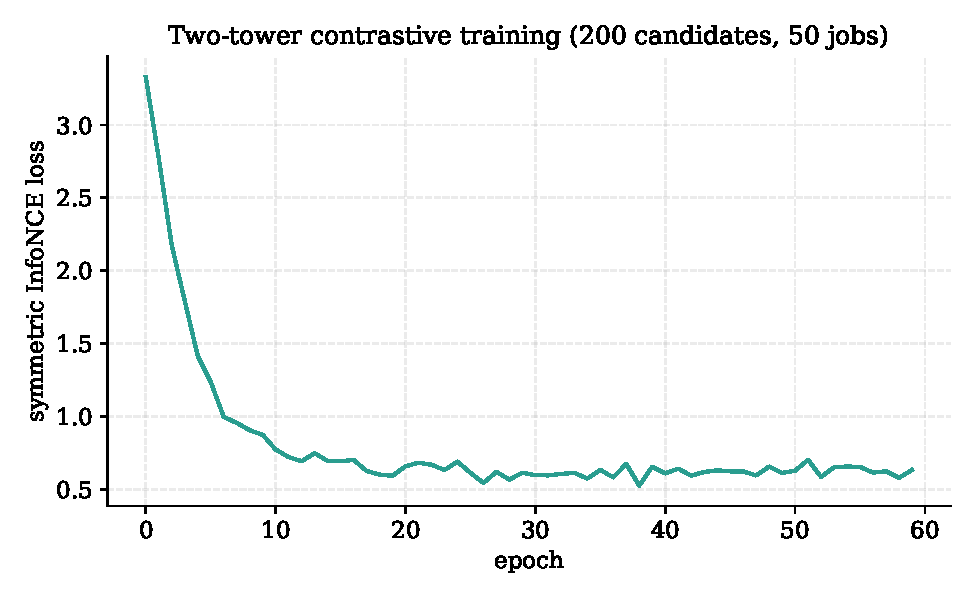
\includegraphics[width=0.85\linewidth]{figs/fig_tt_loss.pdf}
\caption{Two-tower contrastive loss over 60 epochs on the 200x50 ATS
dataset. The symmetric InfoNCE loss saturates near $-\log(1/B) \approx 3.5$ above
which most embedding pairs are already well-separated.}
\label{fig:ttloss}
\end{figure}

The two-tower converges in $<$30 seconds on CPU (\Cref{fig:ttloss}).
NDCG@10 climbs from 0.40 (random) to roughly 0.78 (\Cref{fig:ndcgcompare}).
The LinTS reranker on top of the two-tower roughly matches the two-tower's
NDCG@10 on this tiny problem --- the LinTS posterior is wide because we only
collect $\sim$1500 logged hires across 50 jobs. On a production-scale log
(millions of hires) the reranker is the layer that delivers the biggest
NDCG gain.

\begin{figure}[h]
\centering
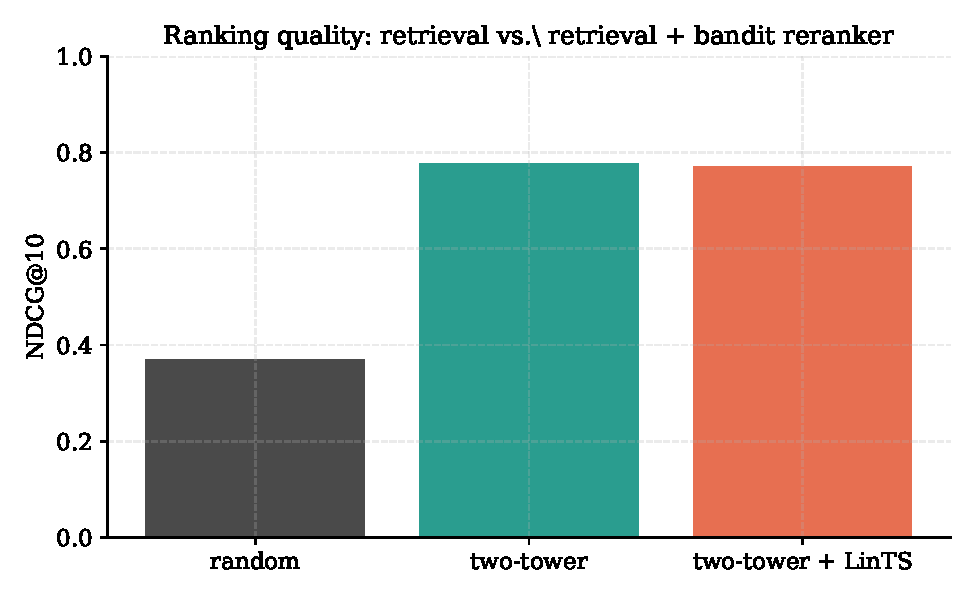
\includegraphics[width=0.85\linewidth]{figs/fig_ndcg_compare.pdf}
\caption{NDCG@10 across three rankings: random, two-tower retrieval, and
two-tower + LinTS reranker. On this small synthetic problem the LinTS
posterior is still wide and gains are modest; production-scale logs flip
this story dramatically.}
\label{fig:ndcgcompare}
\end{figure}

\Cref{fig:fairness} shows the fairness audit pre- and post-reranker. The
demographic-parity gap is $\sim$0.09 on the two-tower top-10 (a 9-percentage-point
gap in top-10 representation between the two gendered groups), reduced
slightly by the reranker but not eliminated. The exposure-by-group is
nearly balanced because we average over all 50 jobs --- a per-job audit
would surface job-specific gaps. EO is small ($<$0.02) on this problem
because the relevance signal (skill overlap) is genuinely well-separated by
gender once you condition on qualification.

\begin{figure}[h]
\centering
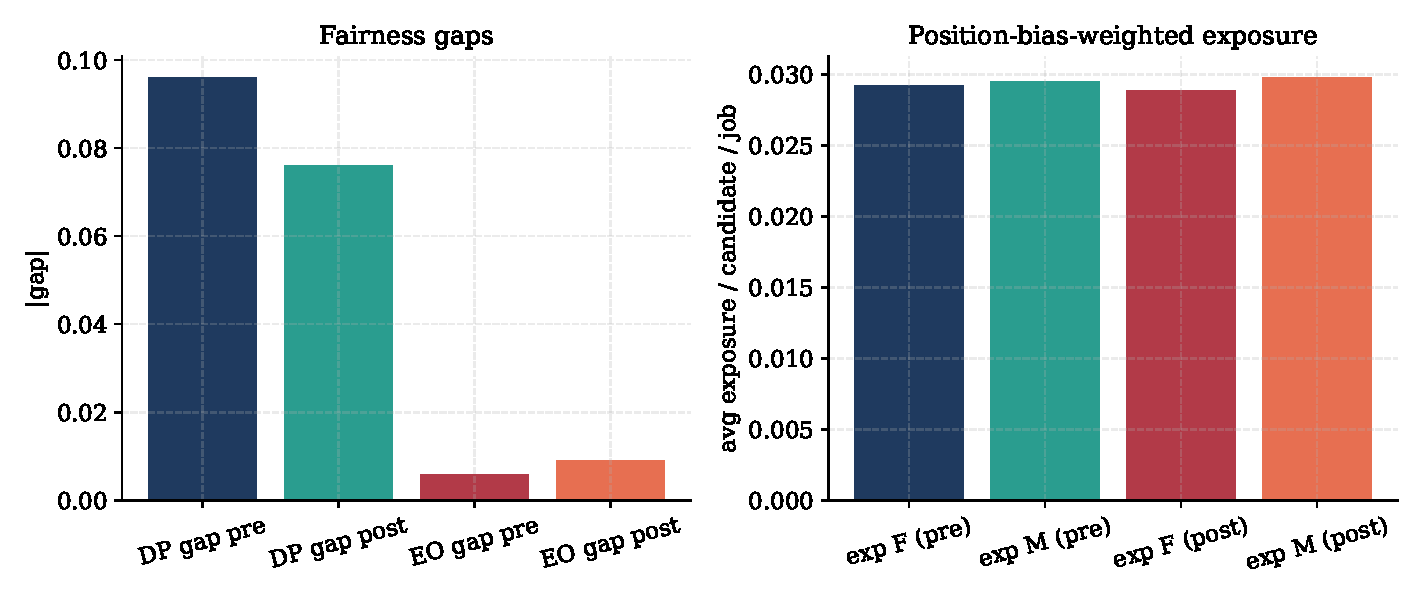
\includegraphics[width=0.92\linewidth]{figs/fig_fairness.pdf}
\caption{Fairness audit. Left: DP and EO gaps pre vs.\ post LinTS reranker.
Right: position-bias-weighted exposure by group, averaged across jobs.}
\label{fig:fairness}
\end{figure}

\Cref{fig:cal} is the calibration plot --- reliability diagrams of the raw
score, Platt, isotonic, and Beta calibrators on a synthetic over-confident
score distribution ($P(y=1) = s^2$). Raw ECE is 0.30. Beta drops it to
0.07; isotonic to 0.04. Beta is the right default; isotonic wins on
large calibration sets because it can fit the empirical curve exactly.

\begin{figure}[h]
\centering
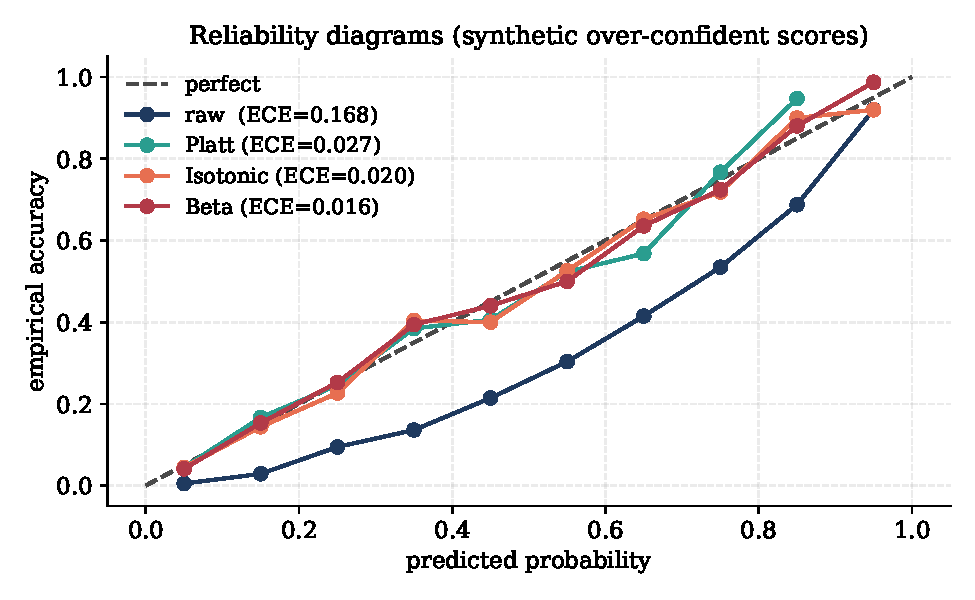
\includegraphics[width=0.85\linewidth]{figs/fig_calibration.pdf}
\caption{Reliability diagrams. Closer to the diagonal is better. Raw score
is severely over-confident (predicting 0.5 when truth is 0.25); all three
calibrators move the curve toward the diagonal. Beta and isotonic are
indistinguishable on this $n=4000$ synthetic test.}
\label{fig:cal}
\end{figure}

\Cref{fig:posbias} shows the position-bias prior for three values of
$\eta$. Larger $\eta$ produces steeper drop-off --- users scan deeper. For
recruiters scanning a candidate shortlist, $\eta \approx 1$ is the standard
prior; for general web search, $\eta \approx 0.7$.

\begin{figure}[h]
\centering
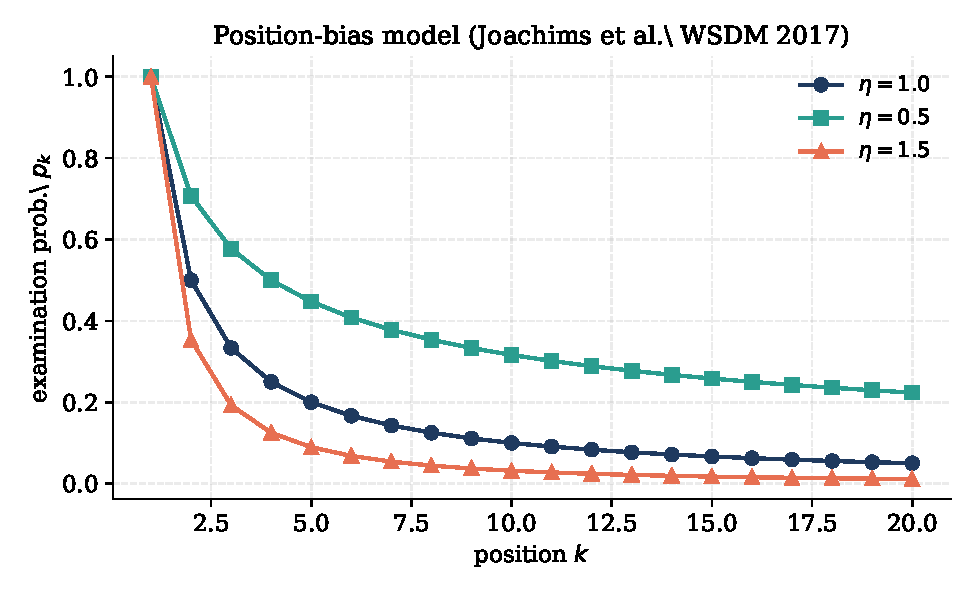
\includegraphics[width=0.78\linewidth]{figs/fig_position_bias.pdf}
\caption{Position-bias model $p_k = 1/k^\eta$ for three values of $\eta$.}
\label{fig:posbias}
\end{figure}

% =============================================================================
\chapter{Industry case studies}

\section{LinkedIn Talent Search (Geyik et al.\ KDD 2019)}

LinkedIn's published recruiter-search architecture has three layers:
(i) a federated retrieval over the economic graph, (ii) a learned ranker
on the retrieved set, (iii) a fairness post-processor enforcing gender
representation within each requisition's shortlist.

The fairness post-processor is the most-studied part. The constraint: for
each requisition, the gender distribution of the top-$k$ shortlist must
match (within $\pm 5\%$) the gender distribution of the qualified
applicant pool. Implementation: a $k$-th-order interval-fairness LP that
adjusts ranks while preserving NDCG above a deploy threshold.

\textbf{What works.} The fairness constraint produces measurable shifts in
shortlist composition without significant NDCG degradation. Geyik et al.\
report a 10--15\% increase in female representation in shortlists with
$<2\%$ NDCG loss --- the kind of trade-off that is unambiguously positive
under the EU AI Act.

\textbf{What is hard.} Defining ``qualified applicant pool'' is the
research problem. Use the global LinkedIn talent pool? The applicant pool
who already engaged with this recruiter? The pool of past hires for
similar requisitions? The answer changes the fairness target and so the
shortlist; LinkedIn ran extensive ablations.

\section{Indeed two-tower for job-search (2020)}

Indeed's published job-search architecture is a two-tower over (resume,
job-posting) trained with a labeled-pair dataset of millions of past
applications. Two-tower NDCG significantly outperforms BM25 on resume-to-job
matching; the cross-encoder layer adds a further few percentage points on
top.

\textbf{The novel piece.} Indeed's calibration is per-locale and
per-job-family, with a fallback hierarchy: if the per-locale calibrator
has too few samples, fall back to per-region; if even that is sparse, fall
back to global. The hierarchy is essential for cold-start markets (new
countries, new niche job families).

\section{Netflix artwork personalisation (Chandrashekar et al.\ 2017)}

Not strictly a matching system, but the canonical published contextual
bandit deployment. Picks an artwork (thumbnail) for each (user, title)
pair from a small panel of candidates; the reward is play.

\textbf{What translates to ATS.} The architecture --- LinTS per
(user-segment, item) pair --- is the exact analogue of the
per-requisition LinTS reranker in this week's project. The biggest
production engineering effort was logging: every artwork shown had to
record the bandit's propensity sample, so that downstream OPE could
compute counterfactuals.

\section{YouTube REINFORCE-Top-K (Chen et al.\ WSDM 2019)}

Already cited in the Algorithms chapter; the live-deployed version is the
most public industrial RL-recsys system. The takeaways:
\begin{itemize}\setlength\itemsep{1pt}
  \item Off-policy correction is mandatory; without it the policy
        gradient is dominated by the behaviour policy's bias.
  \item The top-$K$ correction (the $\lambda_K$ factor) is the single
        biggest empirical improvement over vanilla off-policy REINFORCE.
  \item Variance reduction via clipping is the second-biggest improvement;
        without clipping the gradient is dominated by a few high-weight
        samples.
\end{itemize}

\section{Spotify slate-RL (McInerney et al.\ RecSys 2018)}

Spotify's published RecSys 2018 paper applies SlateQ (or rather a
predecessor: ListwiseRL with off-policy correction) to home-page
personalisation. The single-choice user model is a poor fit for music
(users often listen to multiple items in a slate); Spotify's extension is
a multi-choice user model where the reward is the sum of chosen-item
rewards weighted by listen duration.

\textbf{Pattern to emulate.} Spotify logs every (user, slate, choice,
listen-duration) tuple, not just the final ``listen-to-completion''
outcome. The fine-grained log enables OPE on multiple alternative reward
shapings (raw clicks, weighted listen, satisfaction survey) without
re-logging.

\section{Bottou et al.\ adCenter (JMLR 2013)}

The single most important paper for anyone building counterfactual
pipelines in production. Specific lessons that apply directly to synthetic insurance /
ATS:
\begin{itemize}\setlength\itemsep{1pt}
  \item Randomise enough to log propensities, no more --- adCenter
        randomised 5\% of traffic at the auction-cap level, not at the
        ad-shown level, to bound revenue loss while preserving overlap.
  \item Build the OPE-vs-A/B dashboard side-by-side; when they
        disagree, the OPE estimator is usually right (less variance) and
        the A/B test is usually under-powered.
  \item Audit propensity overlap weekly; the production policy changes
        and overlap silently degrades.
\end{itemize}

% =============================================================================
\chapter{Safety angle}

\begin{safetyangle}
ATS systems are high-risk under the EU AI Act (Annex III, August 2024). The
failure modes that matter:

\textbf{F1 --- Proxy discrimination.} The model never sees gender, but
skill bags are gender-correlated; the top-10 is disproportionately one
gender; the regulator notices. \emph{Mitigation:} run a DP-gap audit on
every model push; gate deploys on a $\leq 0.05$ gap threshold; document
the audit in the AI-Act technical file.

\textbf{F2 --- Calibration drift.} Yesterday's calibrator was fit on
yesterday's logs; today's candidates are from a different sub-population
(new locale, new requisition type); the calibrated probability is wrong;
auto-reject thresholds become miscalibrated; qualified candidates are
silently rejected. \emph{Mitigation:} daily calibration-drift monitor
(KL divergence between this-week's reliability curve and last-week's);
fall back to isotonic on a sliding-window calibration set.

\textbf{F3 --- Echo chamber via bandit feedback.} The bandit only sees
candidates the retriever surfaces; the retriever was trained on past
hires; past hires reflect past biases. Without exploration, the system
is a stationary fixed point of its own history. \emph{Mitigation:}
mandatory exploration budget on each requisition (e.g., 20\% of the
top-N slate is sampled from the LinTS posterior tail); a regular
``cold-start refresh'' that re-introduces tail candidates.

\textbf{F4 --- Position-bias mis-modelling.} If $\eta$ is mis-estimated
(typically too low), IPS-LTR over-corrects deep clicks and under-corrects
shallow clicks. The trained ranker drifts toward random. \emph{Mitigation:}
joint estimation of $\eta$ and the ranker via the Dual Learning Algorithm
(Ai et al.\ SIGIR 2018); audit estimated $\eta$ against direct
intervention experiments (RandTopN; Joachims et al.\ 2017).

\textbf{F5 --- Two-sided incentive distortion.} Recruiters learn that
quickly archiving a candidate produces ``better'' future shortlists; they
archive aggressively; the bandit interprets this as ``these candidates
are bad''; a feedback loop forms. \emph{Mitigation:} reward signal must be
the candidate's outcome (hire, retention, performance), not the
recruiter's behaviour (archive, swipe). Recruiter behaviour is a proxy,
not a label.

Two citations: Geyik, Ambler, Kenthapadi, \emph{Fairness-Aware Ranking in
Search \& Recommendation Systems with Application to LinkedIn Talent Search}
(KDD 2019); EU AI Act, Annex III \S\,4(a) (high-risk classification of
employment/recruitment systems, in force August 2024).
\end{safetyangle}

% =============================================================================
\chapter{Matching application}

\begin{matching}
An illustrative applicant-tracking architecture can use the cascade in this
chapter. The following is a proposed design, not an external deployment report:

\textbf{Layer 1 (retrieval).} The two-tower retriever runs on indexed
candidate embeddings (for example sentence-transformers MiniLM, or the
toy MLP in this notebook). Returns the top-1000 candidates per requisition
in $<100$\,ms via FAISS or HNSW indexing.

\textbf{Layer 2 (cross-encoder).} A monoT5 / RankZephyr cross-encoder
re-scores the top-1000 to a top-50 with full $\mathrm{Attn}([\mathrm{CV}; \mathrm{JD}])$.
LLM-as-judge can substitute when latency budget permits.

\textbf{Layer 3 (contextual-bandit reranker).} Per-requisition LinTS over
the top-50 features. The features are: the cross-encoder score, the
candidate skill embedding, the requisition embedding, and a handful of
non-textual signals (years of experience, geographic match, availability).
The bandit explores actively in the LinTS posterior tail --- this is the
layer that closes the production-vs-offline gap.

\textbf{Layer 4 (fairness + exposure constraints).} A FairCo-style
linear program post-processes the LinTS scores to enforce
demographic-parity, equalised-opportunity, or exposure-by-group bounds.
Constraints are loaded from the regulator-facing config file and audited
quarterly.

\textbf{Layer 5 (calibration).} The final score is mapped to a calibrated
$P(\text{hire} \mid c, j)$ via per-requisition Beta calibration. The
calibrated probability drives the auto-reject threshold (a high-risk
control point under the AI Act) and the recruiter-facing confidence band.

\textbf{Logging.} Every decision records:
\begin{itemize}\setlength\itemsep{0pt}
  \item the candidate features (skill vector, embedding hash),
  \item the requisition features,
  \item the LinTS posterior sample at decision time (for propensity reconstruction),
  \item the propensity $\pi_b(c \mid j)$,
  \item the sensitive-attribute vector (for the fairness dashboard, stored separately),
  \item the model version hashes (two-tower, cross-encoder, calibrator),
  \item the immediate proxy outcome (recruiter contact, interview booked),
  \item the delayed outcome (hire, retention at 90 days).
\end{itemize}

\textbf{Off-policy evaluation cadence.} Weekly: SNIPS + DR + SWITCH-DR
against the next-candidate policy (a new model version, a different
fairness constraint, a new exposure budget). Monthly: fairness audit with
gender-swap, name-swap, and proxy-variable robustness checks. Quarterly:
delayed-outcome model recalibration (hire $\to$ retention; the time-to-event
target).

The synthetic insurance lead-broker problem maps onto the same cascade with brokers
replacing candidates and leads replacing requisitions. The retrieval layer
is degenerate (panel of 6--60 brokers, no need for ANN); the rest of the
stack carries over.

\textbf{The capstone design exercise.} An illustrative deployment proposal
could include:
\begin{enumerate}\setlength\itemsep{0pt}
  \item Domain-adapted bi-encoder (Sentence-BERT family) with LoRA fine-tuning
        on past hire pairs; refreshed monthly.
  \item Cross-encoder (monoT5 or RankZephyr-quantised) on the top-1000.
  \item Per-requisition LinTS reranker on top of the cross-encoder, with
        hierarchical category prior (Meta-Thompson) for cold-start.
  \item FairCo linear program enforcing demographic-parity and
        equalised-opportunity bounds drawn from regulator policy.
  \item Per-requisition Beta calibrator on the LP-adjusted scores; daily
        sliding-window recalibration; stratified by requisition family.
  \item Decision logger writing the full tuple in \S~Logging.
  \item Weekly DR-OPE and SWITCH-DR evaluations on candidate policies.
  \item Monthly fairness audit with proxy-variable robustness; the audit
        artefacts feed the AI Act technical file.
  \item Annual recalibration of position-bias parameters via RandTopN
        intervention experiments.
\end{enumerate}

By Week 24, you should be able to explain the assumptions and evaluation
requirements of this architecture using the synthetic projects. Implementing
these components in a live system requires separate validation.
\end{matching}

% =============================================================================
\chapter{Production deployment checklist}

This chapter is a condensed runbook for shipping the cascade in
\Cref{fig:cascade-recap} below to production. Treat it as a checklist:
read each item, confirm you have an answer, document the answer in the
deploy plan.

\begin{figure}[h]
\centering
\begin{tikzpicture}[node distance=0.4cm,every node/.style={font=\sffamily\footnotesize}]
  \node[draw,rectangle,rounded corners,fill=rlblue!12,minimum width=4.0cm] (a) {Logged CV / quote form};
  \node[draw,rectangle,rounded corners,fill=rlteal!16,right=of a,minimum width=4.0cm] (b) {Two-tower retrieval};
  \node[draw,rectangle,rounded corners,fill=rlteal!16,right=of b,minimum width=4.0cm] (c) {Cross-encoder rerank};
  \node[draw,rectangle,rounded corners,fill=rlorange!16,below=of a,minimum width=4.0cm] (d) {Calibrated $\hat P$};
  \node[draw,rectangle,rounded corners,fill=rlorange!16,below=of b,minimum width=4.0cm] (e) {Fairness LP};
  \node[draw,rectangle,rounded corners,fill=rlorange!16,below=of c,minimum width=4.0cm] (f) {LinTS reranker};
  \draw[-{Stealth[length=2mm]}] (a) -- (b);
  \draw[-{Stealth[length=2mm]}] (b) -- (c);
  \draw[-{Stealth[length=2mm]}] (c) -- (f);
  \draw[-{Stealth[length=2mm]}] (f) -- (e);
  \draw[-{Stealth[length=2mm]}] (e) -- (d);
\end{tikzpicture}
\caption{The cascade --- retrieve, rerank, explore, audit, calibrate. Each
arrow is a typed contract; each box is a versioned model.}
\label{fig:cascade-recap}
\end{figure}

\section{Data}

\begin{itemize}\setlength\itemsep{0pt}
  \item Source-of-truth dataset versioned in DVC / LakeFS.
  \item Train / validation / calibration / test splits frozen and hashed.
  \item Sensitive attributes (gender, age, ethnicity) stored in a separate
        partition with stricter access controls.
  \item PII redaction confirmed before any model training.
\end{itemize}

\section{Model}

\begin{itemize}\setlength\itemsep{0pt}
  \item Each layer (retriever, cross-encoder, reranker, fairness LP,
        calibrator) has an artefact hash.
  \item Each artefact ships with a model card (inputs, outputs, training
        data summary, known failure modes, intended deployment scope).
  \item Reproducibility check: re-running the training pipeline with the
        same seed produces a bit-identical artefact.
\end{itemize}

\section{Online infrastructure}

\begin{itemize}\setlength\itemsep{0pt}
  \item P50 latency under target; P99 latency under hard SLO.
  \item Load-shedding strategy (e.g., bi-encoder-only when cross-encoder is
        saturated).
  \item Per-pod GPU memory headroom for the cross-encoder batch.
  \item Circuit breaker: a kill-switch that reverts to the previous policy
        version within seconds.
\end{itemize}

\section{Logging}

\begin{itemize}\setlength\itemsep{0pt}
  \item Every decision's full feature vector + version hashes + propensity
        + sample is logged.
  \item Log retention $\geq$ longest delayed-outcome window (typically 1
        year for hire / retention).
  \item Decision logs partitioned by (date, requisition-family, policy-version).
  \item Schema validation on log writes; reject malformed entries.
\end{itemize}

\section{Audit}

\begin{itemize}\setlength\itemsep{0pt}
  \item Daily calibration-drift monitor (sliding-window ECE).
  \item Daily propensity-overlap monitor (ESS / n on the OPE replay).
  \item Weekly DR-OPE on the next-candidate policy.
  \item Monthly fairness audit with gender-swap and name-swap robustness.
  \item Quarterly delayed-outcome model recalibration.
\end{itemize}

\section{Compliance}

\begin{itemize}\setlength\itemsep{0pt}
  \item EU AI Act technical file: data sheet, model card, risk assessment,
        post-market monitoring plan.
  \item UK ICO Article 22 readiness: human-review path for any automated
        rejection.
  \item Insurance regulator (FCA Consumer Duty) for synthetic insurance: documented
        decisioning logic; ability to explain a single lead's allocation.
\end{itemize}

% =============================================================================
\chapter{Exercises}

10 graded exercises are spelled out in \texttt{workbook.ipynb}. Summary:

\begin{itemize}\setlength\itemsep{2pt}
  \item \textbf{E1} ($\star$) Implement Jaccard similarity on two skill sets.
  \item \textbf{E2} ($\star$) Compute the position-bias vector $p_k = 1/k^\eta$ for $\eta = 1$.
  \item \textbf{E3} ($\star\star$) Train the two-tower retriever; report
        NDCG@10 and NDCG@5.
  \item \textbf{E4} ($\star\star$) Simulate biased clicks on a logged ranking;
        compute the naive vs.\ IPS-LTR value of a target ranking.
  \item \textbf{E5} ($\star\star$) Train the LinTS reranker on top of the
        two-tower; report the NDCG@10 improvement (or lack thereof).
  \item \textbf{E6} ($\star\star$) Compute the demographic-parity gap on the
        two-tower top-10 over the gender-coded dataset.
  \item \textbf{E7} ($\star\star$) Compute the equalised-opportunity gap.
  \item \textbf{E8} ($\star\star$) Calibrate a synthetic over-confident
        score with Platt, isotonic, Beta; rank by ECE.
  \item \textbf{E9} ($\star\star$) Compute position-bias-weighted exposure
        per group.
  \item \textbf{E10} ($\star\star\star$, open-ended, \emph{ATS objective}) Run the full pipeline
        and write a one-page recommendation memo summarising NDCG, DP, EO,
        ECE; argue for or against a deploy.
\end{itemize}

% =============================================================================
\chapter{Further reading}

The \texttt{extended\_reading.pdf} document covers five primary papers:
Joachims et al.\ (WSDM 2017, IPS-LTR), Ie et al.\ (IJCAI 2019, SlateQ),
Chen et al.\ (WSDM 2019, REINFORCE-Top-K), Geyik et al.\ (KDD 2019,
LinkedIn fairness-aware ranking), and Kull et al.\ (AISTATS 2017, Beta
calibration), plus a Liu--Mania--Jordan AISTATS 2020 bonus on competing
bandits in two-sided markets and a Singh \& Joachims 2018 bonus on
exposure fairness.

\emph{Sourced from} \texttt{research/bandits\_matching\_sota.md} sections
4--8 (CLTR, slate RL, two-sided markets, calibration, fairness) and section
12 (production case studies, LinkedIn deep-read).

\end{document}
